\documentclass{fancyslides} 

\usepackage{times}

\graphicspath{{img/}}

%%% Beamer settings (do not change)
\usetheme{default} 
\setbeamertemplate{navigation symbols}{} %no navigation symbols
\setbeamercolor{structure}{fg=\yourowntexcol} 
\setbeamercolor{normal text}{fg=\yourowntexcol} 



%%%%%%%%%%%%%%%%%%%%%%%%%
%%% CUSTOMISATIONS %%%%%%
%%%%%%%%%%%%%%%%%%%%%%%%%


%%%% SLIDE ELEMENTS
\newcommand{\structureopacity}{0.75} %opacity for the structure elements (boxes and dots)
\newcommand{\strcolor}{blue} %elements colour (predefined blue; orange; green)

%%%% TEXT COLOUR
\newcommand{\yourowntexcol}{white}


%%%%%%%%%%%%%%%%%%%%%%%%%
%%% TITLE SLIDE DATA %%%%
%%%%%%%%%%%%%%%%%%%%%%%%%
\fbckg{nexus}
\newcommand{\titlephrase}{Data Warehouse}
\newcommand{\name}{Javier Bonet \\ Joel Catacora \\}
\newcommand{\affil}{Base de datos avanzada}
\newcommand{\email}{}


\begin{document}


\startingslide %this generates titlepage from the data above


\fbckg{negro}
\begin{frame}
\pointedsl{Definición}
\end{frame}


\fbckg{negro}
\begin{frame}
\misc{Data Warehose es una colección de datos orientada a un determinado ámbito, integrado, no volátil y variable en el tiempo, que ayuda a la toma de decisiones en la entidad en la que se utiliza. Se trata, sobre todo, de un expediente completo de una organización, más allá de la información transaccional y operacional, almacenado en una base de datos diseñada para favorecer el análisis y la divulgación eficiente de datos.}
\end{frame}


\fbckg{negro}
\begin{frame}
\itemized{
\item Integrado: Se integran datos provenientes de múltiples fuentes, posiblemente distintas.
\item No volátil: Una vez almacenados los datos en el DW, la información que éstos representan no debe perderse.
\item Variable en el tiempo: La información histórica se mantiene en el DW a lo largo del tiempo.

}
\end{frame}


\fbckg{negro} % Slide background image
\begin{frame}
\misc{
\begin{figure}[h]
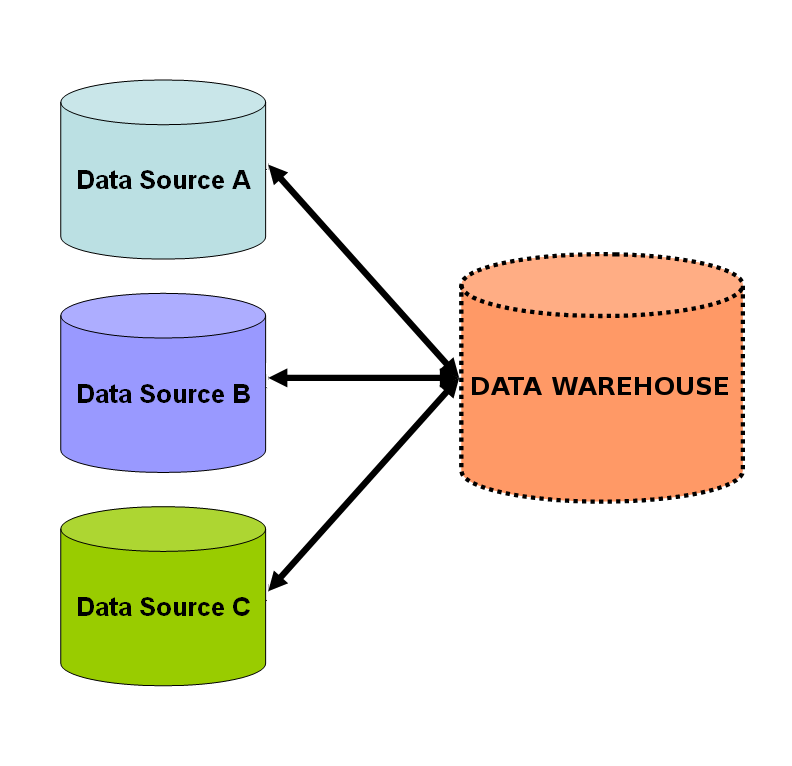
\includegraphics[width=0.7\linewidth]{Dataintegration}
\end{figure}
}
\end{frame}


% \fbckg{blank}
% \begin{frame}
% \framedsl{\pitem{pointed slogan} \pitem{framed slogan} \fitem{beamer features}}
% \end{frame}
% 

% \fbckg{blank}
% \begin{frame}
%   \thankyou   %%%% ending slide with thank you notice
% \end{frame}


% \fbckg{blank}
% \begin{frame}
% \sources{
% \includegraphics[scale=0.048]{1} \ flickr/lovelornpoets\\
% \includegraphics[scale=0.2]{2} \ flickr/apsmuseum
% }
% \end{frame}


\end{document}
